% ----------------------------------------------------------------------
%
%        Vorlage für Abschlussarbeiten am Lehrstuhl Informatik XII
%
%                   http://ls12-www.cs.uni-dortmund.de
%
%   Für Fragen und Anregungen zur Vorlage: info@ls12.cs.uni-dortmund.de
%
%   Stand: 03.09.2013
%
% ----------------------------------------------------------------------
\RequirePackage{ifthen}

\newcommand \type{Fachprojekt Report}
\newcommand \Autor{Lukas B{\"u}nger \\ Thilaksan Kodeeswaran\\ Dilsan Mahadeva}
\newcommand \submissiondate{30.09.2020}
\newcommand \thesistitle{Interactive Real-Time Gaming}
\newcommand \firstsupervisor{Prof.~Dr. Jian-Jia Chen}
\newcommand \secondsupervisor{M.Sc. Junjie Shi}
\newcommand \ErstLehrstuhl{Lehrstuhl Informatik 12 (Eingebettete Systeme) \\ \url{http://ls12-www.cs.tu-dortmund.de}}
\newcommand \ZweitLehrstuhl{}

\RequirePackage{ifpdf} \ifpdf
  \pdfoutput=1
  \pdftrue
  \message{pdfLaTeX}
  \documentclass[pdftex,11pt,a4paper,oneside,ngerman]{scrbook}
  \usepackage[ngerman]{babel}
  \usepackage{float}
  \usepackage[pdftex]{thumbpdf}
  \usepackage[pdftex]{graphicx}
  \usepackage[pdftex]{hyperref}
  \usepackage{pdfpages}
  \pdfoutput=1
  \pdfcompresslevel=9
  \DeclareGraphicsExtensions{.pdf,.jpg,.png}
\else
  \pdffalse
  \message{LaTeX}
  \documentclass[dvips,11pt,a4paper,oneside,ngerman]{scrbook}
  \usepackage{float}
  \usepackage{graphicx}
  \usepackage{epsf}
  \usepackage[dvips]{hyperref}
  \DeclareGraphicsExtensions{.eps}
\fi

% Informationen fuer pdf-File festlegen
\hypersetup
{
    pdfauthor = {\Autor},
    pdftitle = {\thesistitle},
    pdfsubject = {\type, TU Dortmund, Fakult{\"a}t f{\"u}r Informatik},
    pdfproducer = {LaTeX},
    pdfview = FitV,
    pdfstartview = FitV,
    pdfhighlight = /I,
    pdfborder = 0 0 0,
    colorlinks = false,
    bookmarksopen,
    bookmarksopenlevel = 1,
    bookmarksnumbered = false,
    plainpages = false
}%

% -------------------------------------------------------------------
% Seitenformat anpassen
\usepackage[a4paper,left=3.5cm,right=2.5cm,bottom=3.5cm,top=3cm]{geometry}
\setlength{\headheight}{15pt}

% -------------------------------------------------------------------
% Grafikpakete einbinden
\usepackage{amsmath,amssymb}
\usepackage{flafter}
\usepackage{subfigure}

% -------------------------------------------------------------------
\usepackage{ifthen}

% -------------------------------------------------------------------
\usepackage[absolute,overlay]{textpos}
\setlength{\TPHorizModule}{1mm}
\setlength{\TPVertModule}{\TPHorizModule}
\textblockorigin{0mm}{0mm}
\usepackage{fix-cm}
\usepackage{setspace}
\usepackage{scrhack}

% -------------------------------------------------------------------
% Korrekte Darstellung der Umlaute
% \usepackage[german,ngerman]{babel}
% \usepackage[utf8]{inputenc}
% \usepackage[T1]{fontenc}
% \usepackage{ae,aecompl}

% -------------------------------------------------------------------
% Bibtex deutsch
%\usepackage[numbers,sort,square]{natbib}
%\usepackage{bibgerm}

% -------------------------------------------------------------------
% Anführungszeichen
\usepackage[babel,german=quotes]{csquotes}

% -------------------------------------------------------------------
% URLs
\usepackage{url}

% -------------------------------------------------------------------
% Caption anpassen
\usepackage[margin=0pt,font=small,labelfont=bf]{caption}

% -------------------------------------------------------------------
% Erweitere Tabellen
\usepackage{booktabs}

% -------------------------------------------------------------------
% Eurosymbol
\usepackage{eurosym}

% -------------------------------------------------------------------
% Zeilenabstand einstellen
\renewcommand{\baselinestretch}{1.25}
% Floating-Umgebungen anpassen
\renewcommand{\topfraction}{0.9}
\renewcommand{\bottomfraction}{0.8}

% -------------------------------------------------------------------
% Keine einzelnen Zeilen beim Anfang eines Abschnitts ("Schusterjungen")
\clubpenalty = 10000
% Keine einzelnen Zeilen am Ende eines Abschnitts ("Hurenkinder")
\widowpenalty = 10000 \displaywidowpenalty = 10000
\parindent=0cm

% -------------------------------------------------------------------
% Kopfzeile hinzufuegen
\usepackage{fancyhdr}
\usepackage{extramarks}

\pagestyle{fancy}
\renewcommand{\chaptermark}[1]{\markboth{#1}{}}
\renewcommand{\sectionmark}[1]{\markright{#1}{}}

\fancyhf{}
\fancyhead[LE,RO]{\thepage}
\fancyhead[RE]{\textit{\nouppercase{\leftmark}}}
\fancyhead[LO]{\textit{\nouppercase{\rightmark}}}

\fancypagestyle{plain}{ %
\fancyhf{} % remove everything
\renewcommand{\headrulewidth}{0pt} % remove lines as well
\renewcommand{\footrulewidth}{0pt}} \pagestyle{headings}

% -------------------------------------------------------------------
% Eigene Farben definieren
\usepackage{color}
\definecolor{TUGreen}{rgb}{0.517,0.721,0.094}
\definecolor{TUOrange}{rgb}{1.0,0.7176,0.0}
\definecolor{BrightGray}{gray}{0.9}
\definecolor{DarkGray}{gray}{0.2}
\definecolor{white}{rgb}{1,1,1}
\definecolor{black}{rgb}{0,0,0}
\definecolor{red}{rgb}{1,0,0}

% -------------------------------------------------------------------
% Programm-Listings einbinden und formatieren
\usepackage{listings}

\lstdefinestyle{C++}
{
language=C++,
backgroundcolor=\color{BrightGray},
keywordstyle=\tt\bfseries,  %\color{TUGreen}\bfseries,
commentstyle=\color{DarkGray},
stringstyle=\color{red},
showstringspaces=false,
basicstyle=\small\color{black},
numbers=left,
captionpos=b,
tabsize=4,
breaklines=true
}

% -------------------------------------------------------------------
% Algorithmen
\usepackage[plain,chapter]{algorithm}
\usepackage{algorithmic}

\usepackage{enumerate}

% -------------------------------------------------------------------
% Algorithmen anpassen
\renewcommand{\algorithmicrequire}{\textit{Eingabe:}}
\renewcommand{\algorithmicensure}{\textit{Ausgabe:}}
\floatname{algorithm}{Algorithmus}
\renewcommand{\listalgorithmname}{Algorithmenverzeichnis}
\renewcommand{\algorithmiccomment}[1]{\color{grau}{// #1}}

% -------------------------------------------------------------------
% Theorem-Umgebungen
\usepackage[amsmath,thmmarks]{ntheorem}
\theoremseparator{.}
\theoremstyle{change}
\newtheorem{theorem}{Theorem}[section]
\newtheorem{satz}[theorem]{Satz}
\newtheorem{lemma}[theorem]{Lemma}
\newtheorem{korollar}[theorem]{Korollar}
\newtheorem{proposition}[theorem]{Proposition}
% Ohne Numerierung
\theoremstyle{nonumberplain}
\renewtheorem{theorem*}{Theorem}
\renewtheorem{satz*}{Satz}
\renewtheorem{lemma*}{Lemma}
\renewtheorem{korollar*}{Korollar}
\renewtheorem{proposition*}{Proposition}
% Definitionen mit \upshape
\theorembodyfont{\upshape}
\theoremstyle{change}
\newtheorem{definition}[theorem]{Definition}
\theoremstyle{nonumberplain}
\renewtheorem{definition*}{Definition}
% Kursive Schrift
\theoremheaderfont{\itshape}
\newtheorem{notation}{Notation}
\newtheorem{konvention}{Konvention}
\newtheorem{bezeichnung}{Bezeichnung}
\theoremsymbol{\ensuremath{\Box}}
\newtheorem{beweis}{Beweis}
\theoremsymbol{}
\theoremstyle{change}
\theoremheaderfont{\bfseries}
\newtheorem{bemerkung}[theorem]{Bemerkung}
\newtheorem{beobachtung}[theorem]{Beobachtung}
\newtheorem{beispiel}[theorem]{Beispiel}
\newtheorem{problem}{Problem}
\theoremstyle{nonumberplain}
\renewtheorem{bemerkung*}{Bemerkung}
\renewtheorem{beispiel*}{Beispiel}
\renewtheorem{problem*}{Problem}

% Algorithmen anpassen %
\renewcommand{\algorithmicrequire}{\textit{Eingabe:}}
\renewcommand{\algorithmicensure}{\textit{Ausgabe:}}
\floatname{algorithm}{Algorithmus}
\renewcommand{\listalgorithmname}{Algorithmenverzeichnis}
\renewcommand{\algorithmiccomment}[1]{\color{grau}{// #1}}

% Zeilenabstand einstellen %
\renewcommand{\baselinestretch}{1.25}
% Floating-Umgebungen anpassen %
\renewcommand{\topfraction}{0.9}
\renewcommand{\bottomfraction}{0.8}
% Abkuerzungen richtig formatieren %
\usepackage{xspace}
\newcommand{\vgl}{vgl.\@\xspace} 
\newcommand{\zB}{z.\nolinebreak[4]\hspace{0.125em}\nolinebreak[4]B.\@\xspace}
\newcommand{\bzw}{bzw.\@\xspace}
\newcommand{\dahe}{d.\nolinebreak[4]\hspace{0.125em}h.\nolinebreak[4]\@\xspace}
\newcommand{\etc}{etc.\@\xspace}
\newcommand{\evtl}{evtl.\@\xspace}
\newcommand{\ggf}{ggf.\@\xspace}
\newcommand{\bzgl}{bzgl.\@\xspace}
\newcommand{\so}{s.\nolinebreak[4]\hspace{0.125em}\nolinebreak[4]o.\@\xspace}
\newcommand{\iA}{i.\nolinebreak[4]\hspace{0.125em}\nolinebreak[4]A.\@\xspace}
\newcommand{\sa}{s.\nolinebreak[4]\hspace{0.125em}\nolinebreak[4]a.\@\xspace}
\newcommand{\su}{s.\nolinebreak[4]\hspace{0.125em}\nolinebreak[4]u.\@\xspace}
\newcommand{\ua}{u.\nolinebreak[4]\hspace{0.125em}\nolinebreak[4]a.\@\xspace}
\newcommand{\og}{o.\nolinebreak[4]\hspace{0.125em}\nolinebreak[4]g.\@\xspace}
\newcommand{\oBdA}{o.\nolinebreak[4]\hspace{0.125em}\nolinebreak[4]B.\nolinebreak[4]\hspace{0.125em}d.\nolinebreak[4]\hspace{0.125em}A.\@\xspace}
\newcommand{\OBdA}{O.\nolinebreak[4]\hspace{0.125em}\nolinebreak[4]B.\nolinebreak[4]\hspace{0.125em}d.\nolinebreak[4]\hspace{0.125em}A.\@\xspace}

% Leere Seite ohne Seitennummer, naechste Seite rechts
\newcommand{\blankpage}{
 \clearpage{\pagestyle{empty}\cleardoublepage}
}


\begin{document}
% Titelseite ---------------------------------------------------------
%
\pdfbookmark{Titelpage}{pdf:title}
\pagenumbering{alph}
\pagestyle{empty}
%\selectlanguage{german}
\include{chapter/titlepage}
%\blankpage


% Inhaltsverzeichnis -------------------------------------------------
%
\pdfbookmark{Table of Content}{pdf:toc}
\pagenumbering{roman}
\tableofcontents
%\cleardoublepage
\pagenumbering{arabic}

% Inhalte --------------------------------------------------------------
%Einleitung/Motivation/What is RTOS?
%========================================================================================
% TU Dortmund, Informatik Lehrstuhl VII
%========================================================================================

\chapter{Einleitung}
\label{Einleitung}

Hier gehen wir kurz darauf ein, wie das Projekt zustande gekommen ist und in welcher Entwicklungsumgebung gearbeitet wurde.

\section{Motivation und Hintergrund}
\label{Motivation_und_Hintergrund}
%
Durch die Vergabe des Projektes war uns klar ein kleineres Retro Spiel zu programmieren, nach einiger Überlegung und Diskussion zu einfachen aber leicht erweiterbaren Spielen kamen wir auf das Snake. Jedoch war unser Ziel dar{\"u}ber hinaus mehr als nur das klassische Spiel zu implementieren. Es kamen sehr schnell viele Erweiterungsvorschl{\"a}ge wie mehr und variierte Food-Elemente oder spezielle Level oder Mehrspielermodi. Insbesondere gab es sogar noch weitere Ideen zu neuen Leveln und weiteren Spielmodi, die aber wegen zeitlichen Begrenzungen des Projekts vernachl{\"a}ssigt wurden und daf{\"u}r mehr dafür gesorgt wurde, dass die implementierten Erweiterungen reibungslos funktionieren.


\section{Aufbau und Umgebung der Arbeit}
\label{Aufbau_und_Umgebung_der_Arbeit}
%
Die Vorgabe ein Echtzeitbetriebssystem (engl. RTOS) an der Universit{\"a}t im Labor zu nutzen, war wegen der Corona-Pandemie eine unm{\"o}gliche Aufgabe. Auf Grund dessen wurde das gesamte Fachprojekt online abgehalten. Dadurch war ein Emulator, welcher solch ein Echtzeitbetriebssystem simuliert, das Grundwerkzeug und Grundumgebung, womit das Projekt realisiert wurde. Durch das Einarbeiten in den Code des Emulators wurde es mit der Zeit immer verst{\"a}ndlicher den Aufbau des Simulators zu verstehen um das Spiel zu implementieren. Unter anderem hat die Versionsverwaltung mit GitHub die Zusammenarbeit von uns sehr vereinfacht. Dadurch konnte strukturiert und effektiv an dem Projekt gearbeitet werden. Durch den WebClient BigBlueButton konnten wir digitale Treffen abhalten, in denen Probleme und Ideen als Gruppe besprochen wurden. 

%\cleardoublepage
%Game (Game description,Pictures) Thilli
%========================================================================================
% TU Dortmund, Informatik Lehrstuhl VII
%========================================================================================
\chapter{Spiel}
\label{Spiel}
%
In diesem Abschnitt wird das Snake Spiel beschrieben und die Funktionen von Elementen im Gameplay oder Buttons erklärt. Dabei wird gar nicht auf die Implementierung eingegangen, sondern nur erklärt wie das Spiel funktioniert.


\section{Spiel - Hauptmenü}
\label{Spiel_-_Hauptmenü}
%
\begin{figure}[h]
 \centering
 \includegraphics[scale=0.5]{bilder/Hauptmenü}
 \caption{Hauptmenü}
 \label{fig:hauptmenü}
\end{figure}
Das Hauptmenü \ref{fig:hauptmenü} erscheint beim starten des Spiels und hat fünf Buttons. Liegt der Mauszeiger über dem Fragezeichen-Button wird eine Anleitung des Spiels angezeigt. Dort wird die Steuerung für die jeweiligen Spieler angezeigt und spezielle Elemente aus dem Mehrspielermodus erklärt.\\
\begin{minipage}[X]{1.1\textwidth}
 \centering
 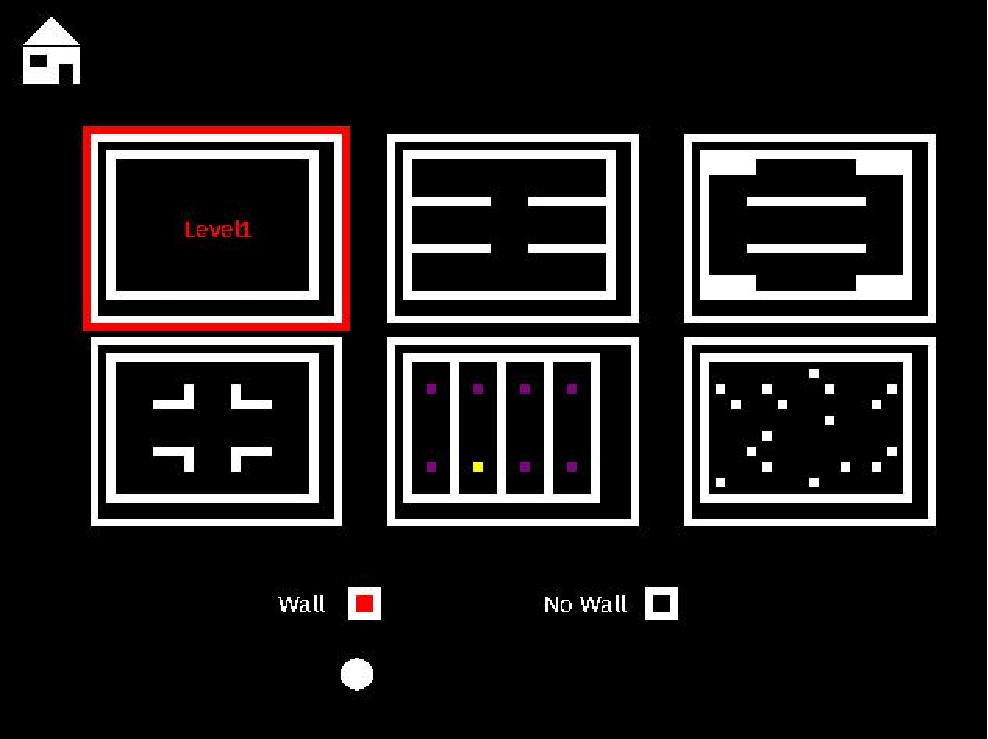
\includegraphics[scale=0.5]{bilder/Einstellungen}
 \captionof{figure}{Einstellungen}
 \label{fig:einstellungen}
\end{minipage}
\newline \\ \\
Wird auf das Zahnrad rechts oben geklickt, öffnet sich das Einstellungsmenü \ref{fig:einstellungen}, indem verschiedene Levels ausgewählt werden können und die Außenwand aktiviert und deaktiviert werden kann. Ist die Außenwand deaktiviert, kann die Schlange beim kollidieren mit der Außenwand nicht sterben. Durch klicken auf das Haus links oben kehrt der Spieler zum Hauptmenü zurück.\newline \newline \\ 
\begin{minipage}[X]{1.1\textwidth}
 \centering
 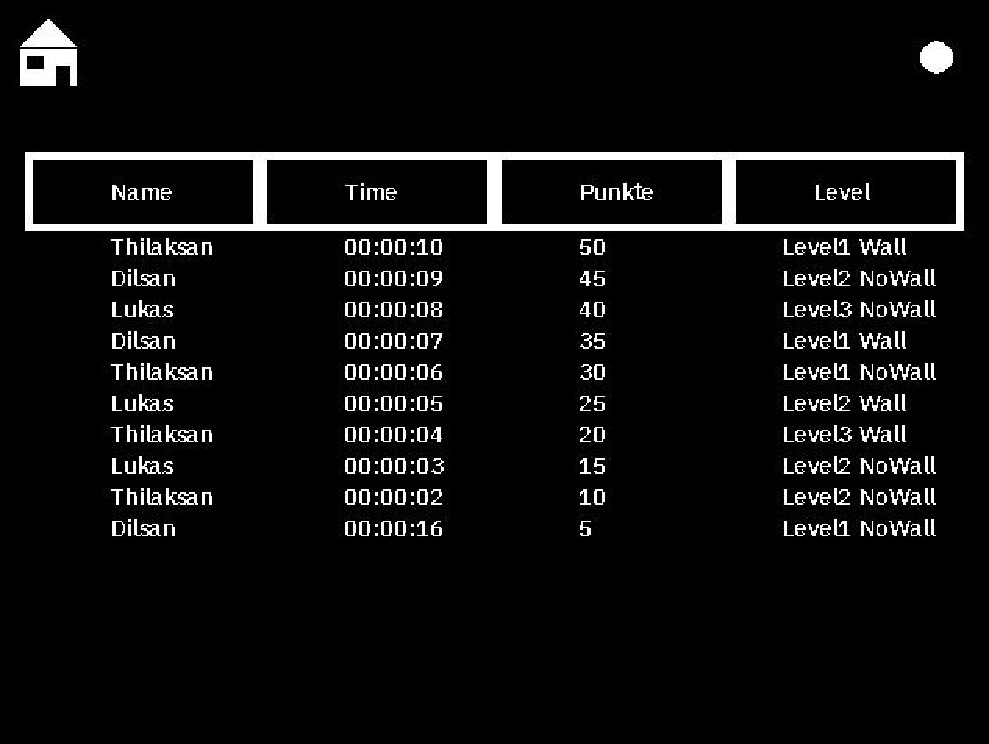
\includegraphics[scale=0.5]{bilder/Highscore}
 \captionof{figure}{Highscore}
 \label{fig:highscore}
\end{minipage}
\newline \\ \\
Wird im Hauptmenü auf den Highscore-Button geklickt, wird der Highscore \ref{fig:highscore} aus den bisher gespielten Spielen angezeigt. Dabei sind die Highscores primär nach Punkten und sekundär nach Zeit sortiert. Außerdem steht in jeweils der letzten Zeile der Highscores das Level, indem gespielt wurde. Mit Klicken auf das Haus links oben kehrt der Spieler zurück zum Hauptmenü.
\\
 Klickt der Spieler auf den "One Player Game"-Button öffnet sich ein Menü, indem der Spieler seinen Namen eintragen kann. Dies kann durch Klicken auf die jeweiligen Buttons auf dem Bildschirm oder durch Eingabe über die Tastatur geschehen. Das Spiel wird dann gestartet, wenn der StartGame-Button betätigt wurde. Wählt der Spieler den Mehrspielermodus, durch Betätigen des "Two Player Game"-Button im Hauptmenü, öffnet sich wieder ein Menü zum Eintragen der Spielernamen und das Spiel kann durch das Betätigen des StartGame-Buttons gestartet werden.  


\section{Spiel - Einzelspielermodus}
\label{Spiel_-_Einzelspielermodus}
%
\begin{figure}[h]
 \centering
 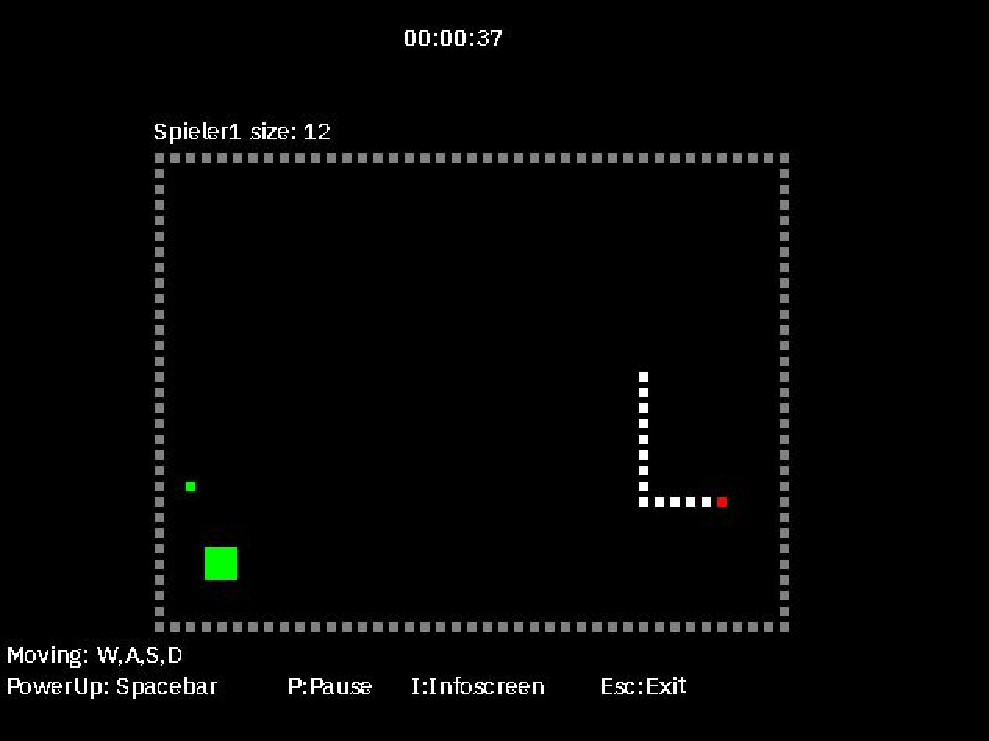
\includegraphics[scale=0.5]{bilder/Einzelspielermodus}
 \caption{Einzelspieler Spiel}
 \label{fig:einzelspielermodus}
\end{figure}
	Der Einzelspielermodus ist im Grunde das traditionelle Snake Game. Die Schlange lässt sich steuern durch Betätigen der Tasten A,S,D,F und bewegt sich alle fünf Frames. Die grünen Elemente sind das Essen der Schlange, welches die Schlange wachsen lässt. Dabei wächst die Schlange um eine Größe beim Verzehren des kleinen Food-Elements und um zwei beim Verzehren des großen Superfood-Elements.
	Das Spiel kann durch die entsprechenden Levels erschwert werden.Level fünf hat ein lilanes Teleport-Element, welches die Schlange zu einem anderen Teleport-Element teleportiert. Dabei teleportieren die oberen Elemente zum nächsten rechten Element und die unteren Elemente zum nächsten linkem Element. Level 6 verändert sein inneres Wandmuster nach dem Verzehren des Food-Elements jedoch nicht nach Verzehren des Superfood-Elements. Das Spiel endet, wenn die Schlange mit der Wand oder mit sich selber kollidiert.   


\section{Spiel - Mehrspielermodus}
\label{Spiel_-_Mehrspielermodus}
%
\textcolor{white}{easily}
\newline 
\begin{minipage}[X]{1.0\textwidth}
 \centering
 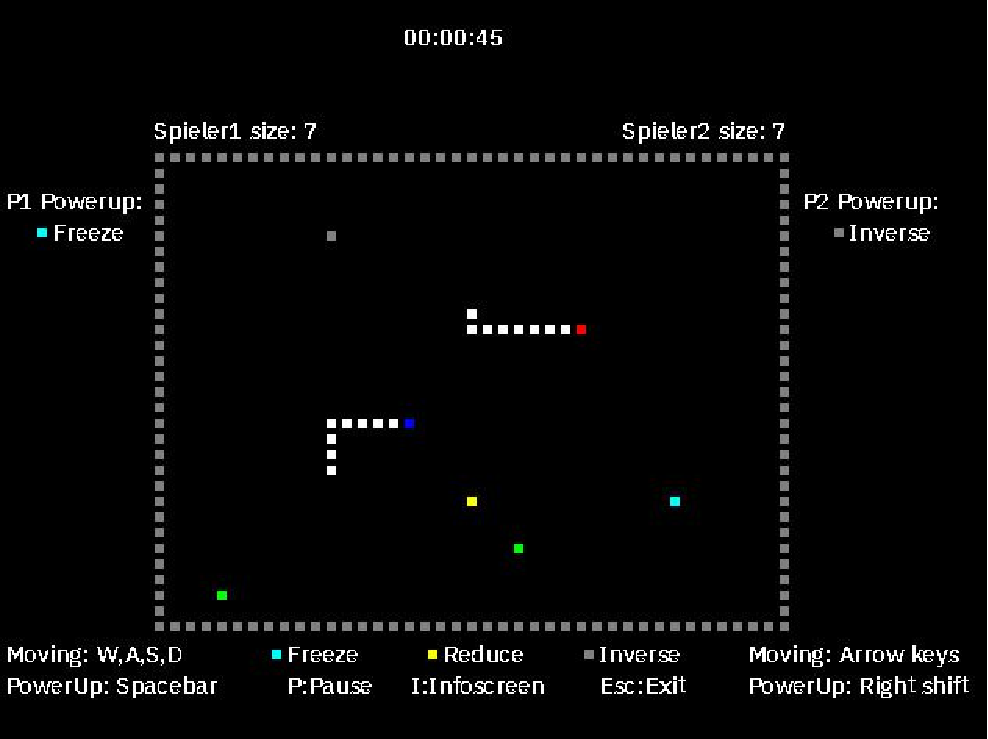
\includegraphics[scale=0.5]{bilder/Mehrspielermodus}
 \captionof{figure}{Mehrspieler Spiel}
 \label{fig:mehrspielermodus}
\end{minipage}
\\ \\ 
	Beim Mehrspielermodus spielen zwei Spieler gegeneinander und versuchen das Spiel durch töten der Schlange des Gegenspielers zu gewinnen. Spieler eins bewegt die rote Schlange mit den Tasten A,S,D,F und Spieler zwei bewegt die blaue Schlange mit den Pfeiltasten. Im Mehrspielermodus gibt es außerdem Spezial-Elemente, wie das cyanfarbene Freeze-Element, das gelbe Reduce-Element und das graue Inverse Element. Diese Elemente können aufgesammelt werden und mit Leertaste für Spieler eins und mit Shift für Spieler zwei eingesetzt werden. Dabei kann nur ein Element gleichzeitig in der Tasche eines jeweiligen Spielers sein. Beim Einsatz des Freeze-Elementes kann die gegnerische Schlange sich für 25 Frames nicht bewegen. Beim Einsatz des Reduce Elementes veringert sich die Länge der gegnerischen Schlange um eine Größe. Das Inverse-Element invertiert die Steuerung des Gegenspielers für 250 Frames. Das Spiel ist beendet, wenn eines der Spieler verliert. Kollidiert die Schlange eines Spielers mit der Wand, sich selber oder dem Körper der gegnerischen Schlange, verliert derjenige Spieler. Kollidieren beide Schlangen Kopf an Kopf gewinnt derjenige Spieler mit der größeren Schlange.  

\section{Spiel - Spielende}
\label{Spiel_-_Spielende}
%
\textcolor{white}{easily}
\newline 
\begin{minipage}[X]{1.1\textwidth}
 \centering
 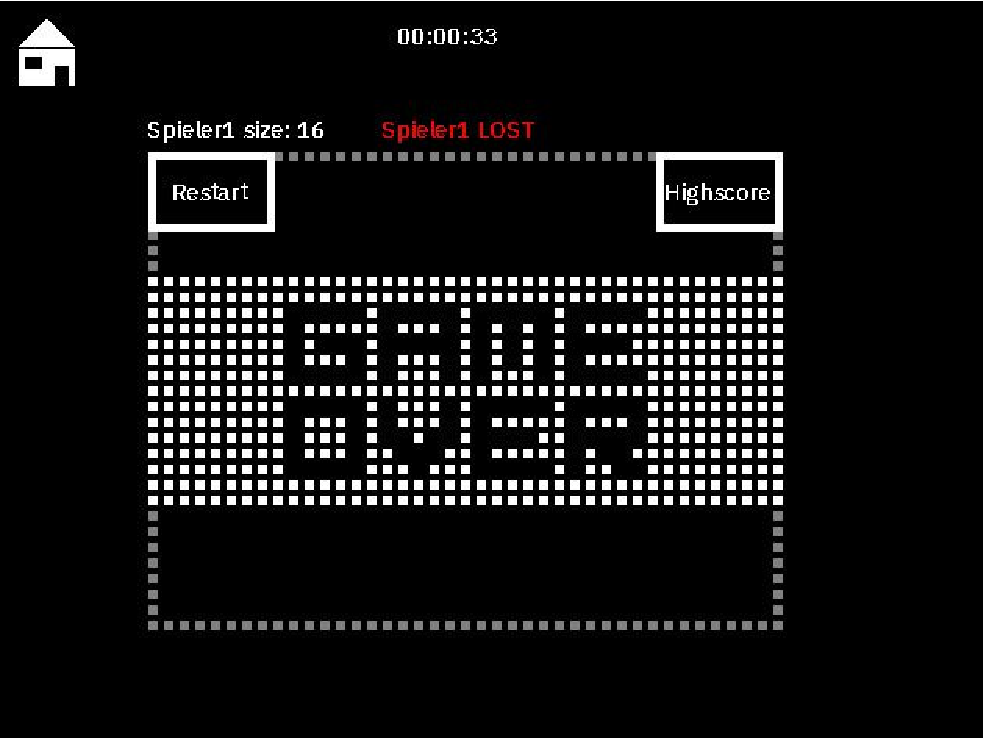
\includegraphics[scale=0.5]{bilder/Spielende}
 \captionof{figure}{Spielende}
 \label{fig:spielende}
\end{minipage}
\\ \\ 
	Ist das Spiel zu Ende erscheint eine kleine Animation und mehrere Buttons. Der Restart-Button startet das Spiel neu und der Highscore-Button zeigt den Highscore an. Außerdem steht über dem Spielfeld welcher Spieler gewonnen hat.  

%


%\cleardoublepage
%Structure ("model structure") Dilsan
%========================================================================================
% TU Dortmund, Informatik Lehrstuhl VII
%========================================================================================

\chapter{Struktur}
\label{Struktur}
%
In diesem Abschnitt wird beschrieben, wie das Spiel in seiner Struktur aufgebaut ist. Dabei werden die Verh{\"a}ltnisse und die Relationen einzelner Elemente miteinander bezogen. 
%

\section{Zust{\"a}nde}
\label{Zustaende}
% 
Das Spiel l{\"a}uft {\"u}ber drei Zust{\"a}nde, da das Spiel {\"u}ber den RTOS-Emulator l{\"a}uft und der Emulator mit Zust{\"a}nden arbeitet. Jeder Zustand arbeitet wie eine Prozess (Task), das bedeutet es kann jeweils nur einer dieser Zust{\"a}nde gleichzeitig arbeiten und die anderen kommen in ein wartenden Bereich. \\
Im erster Zustand wird das Hauptmen{\"u} angezeigt. Dabei werden die Voreinstellungen und die Wahl des Spielmodi gew{\"a}hlt. Obwohl in diesem Prozess verschiedene Anzeigen, wie z.b. Levelauswahl oder Informationbildschirm, des Bildschirms existieren, wird lediglich nur der Bildschirm aktualisiert ohne den Zustand zu wechseln. \\
Der zweite Zustand wird erreicht, indem das w{\"a}hlen des Spielmodis und Eingabe des Names vom Spieler eingegeben wurde. Somit handelt dieser Prozess um das Spiel an sich, das bedeutet, dass die Spielregeln beachtet und jegliche Ver{\"a}derungen im Spiel hier verarbeitet werden. \\
Der letzte Zustand verarbeitet die Rekord bzw. Besten-Liste (Highscore). Hierbei werden die besten zehn Spieler mit den h{\"ochsten} Punkten angezeigt. Dieser Zustand h{\"a}lt die Liste der besten zehn Spieler auf dem aktuellsten Stand und diese Daten werden in einer Datei (\glqq Highscore.txt\grqq{}) gespeichert und exportiert. Insbesondere wird die Datei auch importiert zum Ausgeben der besten Spieler. \\
Jeder Zustand kann durch klicken von Kn{\"o}pfen erreicht werden und der Spieler merkt diese {\"U}berg{\"a}nge in der Regel nicht.
%

%
\section{Verh{\"a}ltnisse der Elemente}
\label{Verhaeltnisse_der_Elemente}
%
Die Verh{\"a}tnisse der Elemente werden im Bezug zu den Zust{\"a}nde beschrieben. \\
Im Hauptmen{\"u} werden Elemente wie Kn{\"o}pfe und Symbole verwendet. Durch dr{\"u}cken eines der Kn{\"o}pfe k{\"o}nnen mehrere Informationen den Nutzer angezeigt werden. Dabei wird der Bildschirm lediglich erneuert, indem der Hintergrund neu gef{\"u}llt wird und dann die neuen Informationen dargestellt. Dasselbe geschieht mit den Voreinstellung des Levels. Die Maus ist auf dem Bildschirm von der Darstellungsebene ganz vorne gesetzt, da die Maus {\"u}ber jedes Objekt sein kann. Entsprechend falls die Maus sich {\"u}ber einer der Kn{\"o}pfe befindet, {\"a}ndert sich die Farbe des Knopfes in grau, um visuell zu zeigen, dass die Maus sich in diesem Bereich befindet. \\ 
Der Highscore Zustand arbeitet sehr {\"a}hnlich wie das Hauptmen{\"u}. Falls sich die Liste {\"a}ndert wird der Bildschirm mit dem Hintergrund neugef{\"u}llt und die Liste danach visualisiert. Jedes mal beim betreten dieses Zustandes wird die Liste durch die Datei \glqq Highscore.txt\grqq{} importiert um die aktuellste List darzustellen. \\
Im Spiel werden mehrere Elemente verwendet, wie z.B. das Food-Element, das Wandelement, die Schlange und das Inventar des Spielers. Dabei ist klar je nach Voreinstellung, dass bei einer Kollision von der Schlange mit der Wand, das Spiel zu Ende sein kann. Damit ist die Schlange untergeordnet als die Wandelemente. Insbesondere ist die Schlange auch innerhalb des Spielfeldes von der Wand eingeschlossen. Im Fall das die W{\"a}nde deaktiviert wurden, springt die Schlange einfach in die gegen{\"u}berliegende Spielfeldseite. Das Teleport-Element in Level 5 besitzt den selben Rang wie die Wandelemente, da durch zusammentreffen mit der Schlange, die Schlange nur an einer anderen Position verschiebt wird. Dagegen sind die PickUp-Elemente wie Food-Element, SuperFood-Element, Decrease-Element, Freeze-Element und Invert-Element von der Schlange abh{\"a}ngig, weil die Schlange diese Elemente aufnehmen kann. Dar{\"u}berhinaus d{\"u}rfen die PickUp-Elemente nicht auf der Schlange erzeugt werden, somit sind diese untergeordnet als die Schlange. Die jeweiligen Schlangen haben jeweils eine Liste als Datenstruktur, damit es einfacher ist Elemente hinzuzuf{\"u}gen und zu entfernen. Durch aufnehmen der Elemente werden einige in ein Inventar gepackt, dabei werden immer die letzten aufgenommen Elemente behalten. Diese Elemente werden jeweils an der Seite des Spielers angezeigt. 

 
%

%\cleardoublepage
%Game Logic Lukas
%========================================================================================
% TU Dortmund, Informatik Lehrstuhl VII
%========================================================================================

\chapter{Spiellogik}
\label{Spiel_Logik}
%
In diesem Kapitel gehen wir auf die Hauptfunktion des eigentlichen Spielablaufs, $vGameScreen()$, und der daf{\"u}r ben{\"o}tigten einzelnen Funktionen ein. Wie in den meisten Computerspielen besteht die Hauptfunkion im groben aus einer einzigen gro{\ss}en Schleife, in der zum der aktuelle Spielzustand abh{\"a}ngig von den Eingaben der Spieler ge{\"a}ndert wird, und zum anderen der aktuelle Spielzustand grafisch aufgearbeitet und auf den Bildschirm gebracht wird. Vor dem Start dieser Schleife findet noch eine Initialisierung statt, welche den Spielzustand auf den Anfang des Spiels setzt.
%

\section{Initialisierung}
\label{Initialisierung}
%
Das erste, was nach Starten des Spiel geschieht, ist das Erstellen eine Art $seed$ f{\"u}r die $rand()$ Funktion der C - Programmiersprache. Da die $rand()$ Funktion die verstrichene Zeit seit Aufruf der Funktion in der sie aufgerufen wird als Basis f{\"u}r die Berechnung der Pseudozufallszahl nimmt, die ersten Aufrufe der $rand()$ Funktion immer die gleichen Werte zur{\"u}ckgeben, und somit die Schlangen der Spieler sowie das erste $foodElement$ immer an der gleichen Stelle starten. Um den entgegenzuwirken berechnet die Funktion als erstes die letzten beiden Ziffern des Produkts der x- und y-Koordinaten der Mausposition beim klicken des Start-Buttons und dekrementiert diese Zahl bis zur null. Durch diese minimale verstrichene Zeitspanne {\"a}ndern sich die Ergebnisse der ersten $rand()$-Aufrufe und damit der Startzustand des Spielfelds, vorrausgesetzt man dr{\"u}ckt beim Start nicht auf den exakt gleichen Pixel wie vorher.
Anschlie{\ss}end werden, je nach gew{\"a}hltem Level, die W{\"a}nde sowie alle weiteren festen Elemente des Levels an ihre entsprechenden Stellen ins $fieldArray$ geschrieben.
Daraufhin werden die Variablen f{\"u}r die Position der beiden Spieler, $p1X, p1Y, p2X$ und $p2Y$, sowie das erste $foodElement$, auf zuf{\"a}llige Positionen im Spielfeld gesetzt. Dafür werden die beiden Funktionen $getRandomFreeField$, welche mit der Methode beschrieben im Kapitel \ref{Elemente Erzeugen}  : \nameref{Elemente Erzeugen} eine freie Stelle auf dem Spielfeld zurückgibt, und $createRandomFood()$, welches auf einer zufälligen Stelle des Feldes ein $foodElement$ erschafft, also die zugehörige Stelle im $fieldArray()$ mit der Nummer $10$ beschreibt sowie die Variablen $food1X, food1Y$ bzw. $food2X, food2Y$ auf die zugehörigen Koordinaten auf dem Bildschirm setzt. Außerdem werden die zugeh{\"o}rigen verketteten Listen f{\"u}r die Schlangen mit bereits 2 weiteren "Schlangenteilen" initialisiert. Dies geschieht auch im Singleplayer-Modus f{\"u}r die Schlange von Spieler 2, da der Code ansonsten aufgrund einer m{\"o}glicherweise nicht initialisierten Spieler-2-Schlange nicht kompiliert. Einzig der Eintrag im $fieldArray()$  wird im Singleplayer-Modus ausgelassen, da offensichtlich kein Spieler 2 existiert.
Zum Schluss werden noch die boolean-Variablen $p1Ready$ und $p2Ready$ auf $false$ sowie $initial$ auf $true$ gesetzt. Diese werden in der nun startenden Hauptschleife benötigt.
Jetzt ist das Spielfeld soweit initialisiert, dass das eigentliche Spiel beginnen kann.
%

\section{Hauptschleife}
\label{Hauptschleife}
%
Wenn das Spiel fertig initialisiert ist startet die Hauptschleife. Da die Variable $initial$ in der Initialisierung auf $false$ gesetzt ist, startet das Spiel nicht direkt, statdessen wird nur der Startzustand, also die Startposition der Schlange sowie die ersten $foodElemente$ angezeigt, sowie eine kurze Animation gezeigt, in der das Level gezeichnet wird. Dadurch können sich die Spieler zuerst mit dem Level vertraut machen und können in Ruhe ihre Startrichtung ausmachen, so dass das Spiel erst startet wenn alle bereit sind. Wenn nun der oder die Spieler eine ihrer Richtungstasten betätigen, wird zum einen die Startrichtung für die Schlangen gesetzt, sowie die zum jeweiligen Spieler gehörige $ready$-Variable auf $true$ gesetzt. Erst wenn die $ready$-Variablen aller Spieler auf $true$ stehen, wird die $initial$-Variable auf $false$ gesetzt und das eigentliche Spiel startet, die Schlangen fangen an sich zu bewegen. Sollte zu diesem Zeitpunkt die Animation des Levels noch nicht abgeschlossen sein, so wird diese abgebrochen und das Level einfach direkt vollständig angezeigt.
Wenn dies alles geschehen ist startet das eigentliche Spiel, und es geschieht jeden Schleifendurchlauf das gleiche, solange bis das Spiel endet in dem einer der Spieler verliert.
Zuerst wird der Zustand der Tastatur durch die Funktion $xGetButtonInput()$ abgerufen, sodass basierend auf den Tastatur-Eingaben der neue Spielzustand berechnet werden kann. Die beiden Funktionen $pause()$ und $infoscreen()$ steuern das pausieren oder weiterführen des Spiels nach dem Drücken der Taste "P" sowie das anzeigen oder verstecken des Hilfe-Textes am unteren Rand des Bildschirms nach Drücken der Taste "I". Mit der Funktion $incrementSpeed()$ überprüft das Spiel, ob einer der Spieler die größe 25, 50, 75 oder 100 erreicht hat, und falls ja, erhöht es die Spielgeschwindigkeit. Die Funktion $checkGameOver$ überprüft, ob einer der Kriterien für ein Ende des Spiels erfüllt sind, also ob einer der Spieler verloren hat. Ist dies der Fall stoppt die Funktion die Bewegung der Schlangen und startet die Game-Over-Animation und zeigt die Button für einen Neustart, die Highscoreliste und das Hauptmenü ein. Außerdem wird, falls ein Highscore erreicht wurde, dieser in die Highscoreliste eingetragen.
Anschließend wird mit $playerOneGetNextDirection()$ bzw $playerTwoGetNextDirection()$ die nächste Richtung der Schlangen bestimmt, wieso dafür eine extra Funktion benutzt wird erklären wir in Kapitel \ref{Bewegung der Schlange}  : \nameref{Bewegung der Schlange}.
Der anschließende Teil der Hauptschleife hängt von den beiden Variablen $frame$ und $frameTicks$ ab. $frame$ gibt die aktuelle Zahl der Schleifendurchläufe seit dem letzten Schritt der Schlangen an und wird somit nach jedem Schleifendurchlauf inkrementiert, während frameTicks die Zahl der benötigten Schleifendurchläufe für einen Schritt angibt. Wenn also $frame == frameticks$ gilt, führen die Schlangen einen Schritt aus und $frame$ wird wieder auf 0 gesetzt. Mit Hilfe dieser beiden Variablen werden auch weitere Elemente des Spiel gesteuert: Wenn das Spiel pausiert oder verloren ist wird $frame$ nicht weiter erhöht damit die Schlangen stehenbleiben, und zur Erhöhung der Laufgeschwindigkeit der Schlangen wird $frameticks$ von anfänglich 5 immer weiter dekrementiert. Wenn im Schleifendurchlauf nun $frames == frameticks$ gilt, geschieht folgendes: Aller Spieler machen mit der Funktion $playerStep()$ einen Schritt in ihre jeweiligen Richtungen. Dabei wird der Kopf der Schlange um eine Einheit in die aktuelle Richtung bewegt, ein neues Schlangenelement an der Stelle an der der Kopf war der Schlange hinzugefügt und die Stelle im $fieldArray$ mit der Spielernummer beschrieben, sowie das letzte Element der Schlange gelöscht und ihre zugehörige Stelle im $fieldArray$ wieder auf 0 gesetzt. Anschließend wird mit der Funktion $collisionDetection()$ überprüft, ob eine der Schlangen mit ihrem letzten Schritt mit etwas zusammengestoßen ist. Dafür wird der Wert des $fieldArray$ an der Stelle des Kopfes überprüft. Ist dieser Wert 1, 2 oder 3, hat der Spieler entweder die Schlange von Spieler 1 oder Spieler 2 oder die Wand getroffen und hat damit verloren. Aber auch das Aufsammeln eines $foodElements$ oder eines $PowerUps$ wird mit der Funktion überprüft. Bevor zum Schluss die Variable $frame$, wie vorher beschrieben, auf 0 gesetzt wird, wird mit der Funktion $powerUps()$ der Einsatz der einzelnen $PowerUps$ überprüft. Diese Mechanik erkläre ich im nachfolgenden Unterkapitel.
Danach muss nurnoch der aktuelle Spielzustand auf dem Bildschirm gez	eichnet werden ($drawBoard()$) und, falls nach Spielende der entsprechende Button gedrückt wurde, zum Hauptmenü zurückgekehrt werden ($backToMenu()$)
%


\section{PowerUps}
\label{PowerUps}
%
Es gibt 3 PowerUps im Spiel, welche während des Spiels von den Spielern aufgesammelt und dann aktiviert werden können, wordurch sie verbraucht werden und folgende Effekte auf die gegnerische Schlange haben: Einfrieren, Umkehrung der Steuerung oder Verkürzung der Schlange. Für alle 3 PowerUps gibt es jeweils einzelne $-exists, -X, -Y$ und $-Player$ Variablen, welche jeweils angeben, ob das jeweilige PowerUp aktuell existiert, deren X- und Y-Koordinaten sowie welcher Spieler aktuell davon betroffen ist. Außerdem gibt es die beiden Variablen $p1PowerUp$ und $p2PowerUp$, welche angeben welches PowerUp jeder Spieler gerade trägt.
Innerhalb der $powerUps()$-Funktion wird zuerst für jedes PowerUp, sowie für das $superFood$-Element, welches ähnlich funktioniert, zuerst überprüft ob es bereits auf dem Spielfeld existiert. Falls nicht, wird eine Pseudozufallszahl berechnet und mit dieser mit einer gewissen Wahrscheinlichkeit (1:50) ein neues PowerUp an einer zufälligen Stelle auf dem Feld erstellt. Falls nun ein Spieler ein PowerUp aufsammelt, was in der $collisionDetection()$ festgestellt und bearbeitet wird, wird die entsprechende PowerUp-Variable des Spielers auf den Wert des PowerUps gesetzt. Wenn nun ein Spieler ein PowerUp besitzt und aktiviert, setzt $powerUps()$ diese Variable wieder auf 0, sowie die entsprechenden Variablen des PowerUps auf ihre Aktivierungswerte. So wird zum Beispiel zum Einfrieren von Spieler 1 $playerOneFrozen$ auf 15 gesetzt. Solange $playerOneFrozen > 0$ gilt, wird für Spieler 1 anstelle eines Schrittes der Schlange der Wert von $playerOneFrozen$ dekrementiert. Die Schlange von Spieler 1 bewegt sich demnach 15 Schritte lang nicht, ist also eingefroren. Ähnlich funktioniert die Invertierung der Steuerung, hierbei wird die Variable $inverseControlOne$ auf 50 gesetzt und mit ebenfalls mit jedem Schritt invertiert. Solange die Variable größer 0 ist, wird in der Funktion $playerOneGetNextDirection()$ die entgegengesetzte Richtung der eigentlich per Tastendruck angegebenen als $nextDirection$ gesetzt. Das Reduzieren der Schlange funktioniert mit gleicher Weise, hierbei wird lediglich die Variable auf 1 gesetzt und im nächsten Schritt wieder zurück auf 0 gesetzt, zusammen mit der Verkürzung der Schlange. 
%


%\cleardoublepage
%Problems and Solutions
%========================================================================================
% TU Dortmund, Informatik Lehrstuhl VII
%========================================================================================

\chapter{Probleme und L{\"o}sungen}
\label{Probleme_und_Loesungen}
%
Im folgendem werden einige Probleme, die bei der Implementierung des Projektes aufgekommen sind, beschrieben und des weiteren werden verschiedene L{\"o}sungsans{\"a}tze dazu vorgestellt.

\section{Bewegung der Schlange}
\label{Bewegung der Schlange}
%
Bei der Implementierung der Schlange wurde am Anfang erst ein Quadrat erstellt, danach musste die Bewegung hinzugef{\"u}gt werden. Da am Anfang noch keine Bildschirmrate gab, konnte die Schlange in jede Richtung in Echtzeit laufen, je nach Eingabe der Richtung. Um die Schlange in direkter Diagonalen Richtungen zu vermeiden, wurde die Bewegung in Horizontaler- und Vertikaler-Achse beschr{\"a}nkt. Das Problem war, dass die Schlange in die entgegengesetzte Richtung laufen kann, d.h. die Schlange konnte durch sich selbst durchlaufen.

Der erste L{\"o}sungsansatz war mit Hilfe von einer Variable die aktuelle Richtung zu speichern um je nachdem in die andere Achse zu laufen. Damit wird verhindert direkt in die entgegengesetzte Richtung zu laufen. Jedoch wurde das Problem noch nicht behoben, da durch das gleichzeitige Benutzen von mehreren Richtungseingaben die Variable eine falsche Richtung erh{\"a}lt und somit die entgegengesetzte Richtung erlaubt. Dies kann so schnell passieren, sodass die Schlange die zweite Richtung nicht wahrnimmt und sofort in die entgegengesetzte Richtung l{\"a}uft.

Deshalb gab es einen endg{\"u}ltigen L{\"o}sungsansatz, welcher mit zwei Variablen und mit der Methode, die jeden Schritt der Schlange verarbeitet, arbeitet. Die Variablen sind dabei einmal $p1Direction$ (f{\"u}r Player1 und Player2 $p2Direction$) f{\"u}r die aktuelle Richtung und $p1NextDirection$ (f{\"u}r Player1 und Player2 $p2NextDirection$) f{\"u}r die n{\"a}chste Richtung. Die Idee mit dem Verhindern der Achse bleibt. Jedoch wird die aktuelle Richtung erst auf die neue Richtung gesetzt, sobald die Schlange sich um ein Feld bewegt. 
%
\section{Elemente Erzeugen}
\label{Elemente Erzeugen}
Relativ fr{\"u}h in der Entwicklung des Spiels machten sich Performanceprobleme beim Erstellen neuer Elemente, vor allem des $foodElement$, bemerkbar. Bei zunehmend langer Schlange erh{\"o}hte sich die Rechenzeit f{\"u}r das Finden einer freien Stelle auf dem Spielfeld so stark, dass zum Beispiel nach dem finden des $foodElements$, eine bemerkbare Pause entstand in der das Spiel nicht weiterlief und somit stockte. Diese Pause war allerdings nicht gleichbleibend lang, sondern erschien zuf{\"a}llig und mit unterschiedlicher Dauer, jedoch mit ansteigender L{\"a}nge der Schlange {\"o}fter und mit erhöhter Dauer.\\
Dies war zur{\"u}ckzuf{\"u}hren auf unseren Algorithmus zur Bestimmung einer freien Stelle sowie die Speicherung der Schlange in einer Liste. Der Algorithmus suchte pseudo-randomisiert eine Stelle des Spielfeldes aus und {\"u}berpr{\"u}fte daraufhin, ob ein Element der Schlange bereits auf diesem Feld ist. Falls dies nicht der Fall war, war das Feld geeignet, ansonsten wurde einfach ein anderes Feld ausgesucht und dies solange wiederholt bis ein freies Feld gefunden wurde. Durch eine l{\"a}ngere Schlange stieg somit die Wahrscheinlichkeit, dass ein neues Feld ausgesucht und der {\"u}berpr{\"u}fungsprozess deshalb mehrere Male durchgef{\"u}hrt werden musste. Das gr{\"o}ßere Problem hierbei war aber der {\"U}berpr{\"u}fungsprozess selber, sowie die Speicherung der Schlange in einer verketteten Liste. Um zu {\"u}berpr{\"u}fen, ob das ausgesuchte Feld nicht schon durch die Schlange belegt war, musste die gesamte Schlange Element f{\"u}r Element {\"u}berpr{\"u}ft werden. In Kombination mit der Wahrscheinlichkeit auf mehrere {\"U}berpr{\"u}fungen entstand dadurch bei l{\"a}ngeren Schlangen ein so großer Rechenaufwand, dass die  Verz{\"o}gerung durch den Spieler bemerkbar und somit der Spielfluss ins stocken geraten ist.\\
Zur L{\"o}sung des Problems wurde eine neue Variable eingef{\"u}hrt, welche auch in der weiteren Entwicklung noch sehr hilfreich wurde: ein zweidimensionales Array mit Integer-Werten, das $fieldArray$. Das $fieldArray$ dient als kompakte Darstellung des aktuellen Zustands des gesamten Spielfelds. Dabei repr{\"a}sentierte jeder der 39 x 29 Integer-Werte eine Stelle auf dem Spielfeld und deren aktuellen Zustand. Ist der Wert 0 ist das Feld frei, ist der Wert 1 ist die Stelle von der Schlange von Spieler 1 belegt usw. . Alle Werte und zugeh{\"o}rigen Zust{\"a}nde sind in Tabelle \ref{tbl:Fieldarray-Werte}zu sehen.
\\
Durch das $fieldArray$ ist nun der Prozess des {\"u}berpr{\"u}fens einer Stelle nicht mehr abh{\"a}ngig von der L{\"a}nge der Schlange, sondern kann immer in konstanter Zeit durch einmaliges checken des zugeh{\"o}rigen Wertes im $fieldArray$ erledigt werden. Das Problem der mehrmaligen {\"u}berpr{\"u}fungen durch Ausw{\"a}hlen eines bereits belegten Feldes ist damit auch trivialisert, da das {\"u}berpr{\"u}fen nun schnell genug geht. Durch das $fieldArray$ wurde auch die weitere Implementierung des Spiels vereinfacht, da durch neue Wertezuweisungen im Array relativ einfach neue Objekte wie W{\"a}nde und PowerUps in die Spiellogik eingef{\"u}hrt werden konnten, und das {\"u}berpr{\"u}fen der Stellen an denen diese Objekte sich befinden durch das $fieldArray$ direkt abgedeckt ist.

\begin{minipage}[X]{1.1\textwidth}
 \centering
 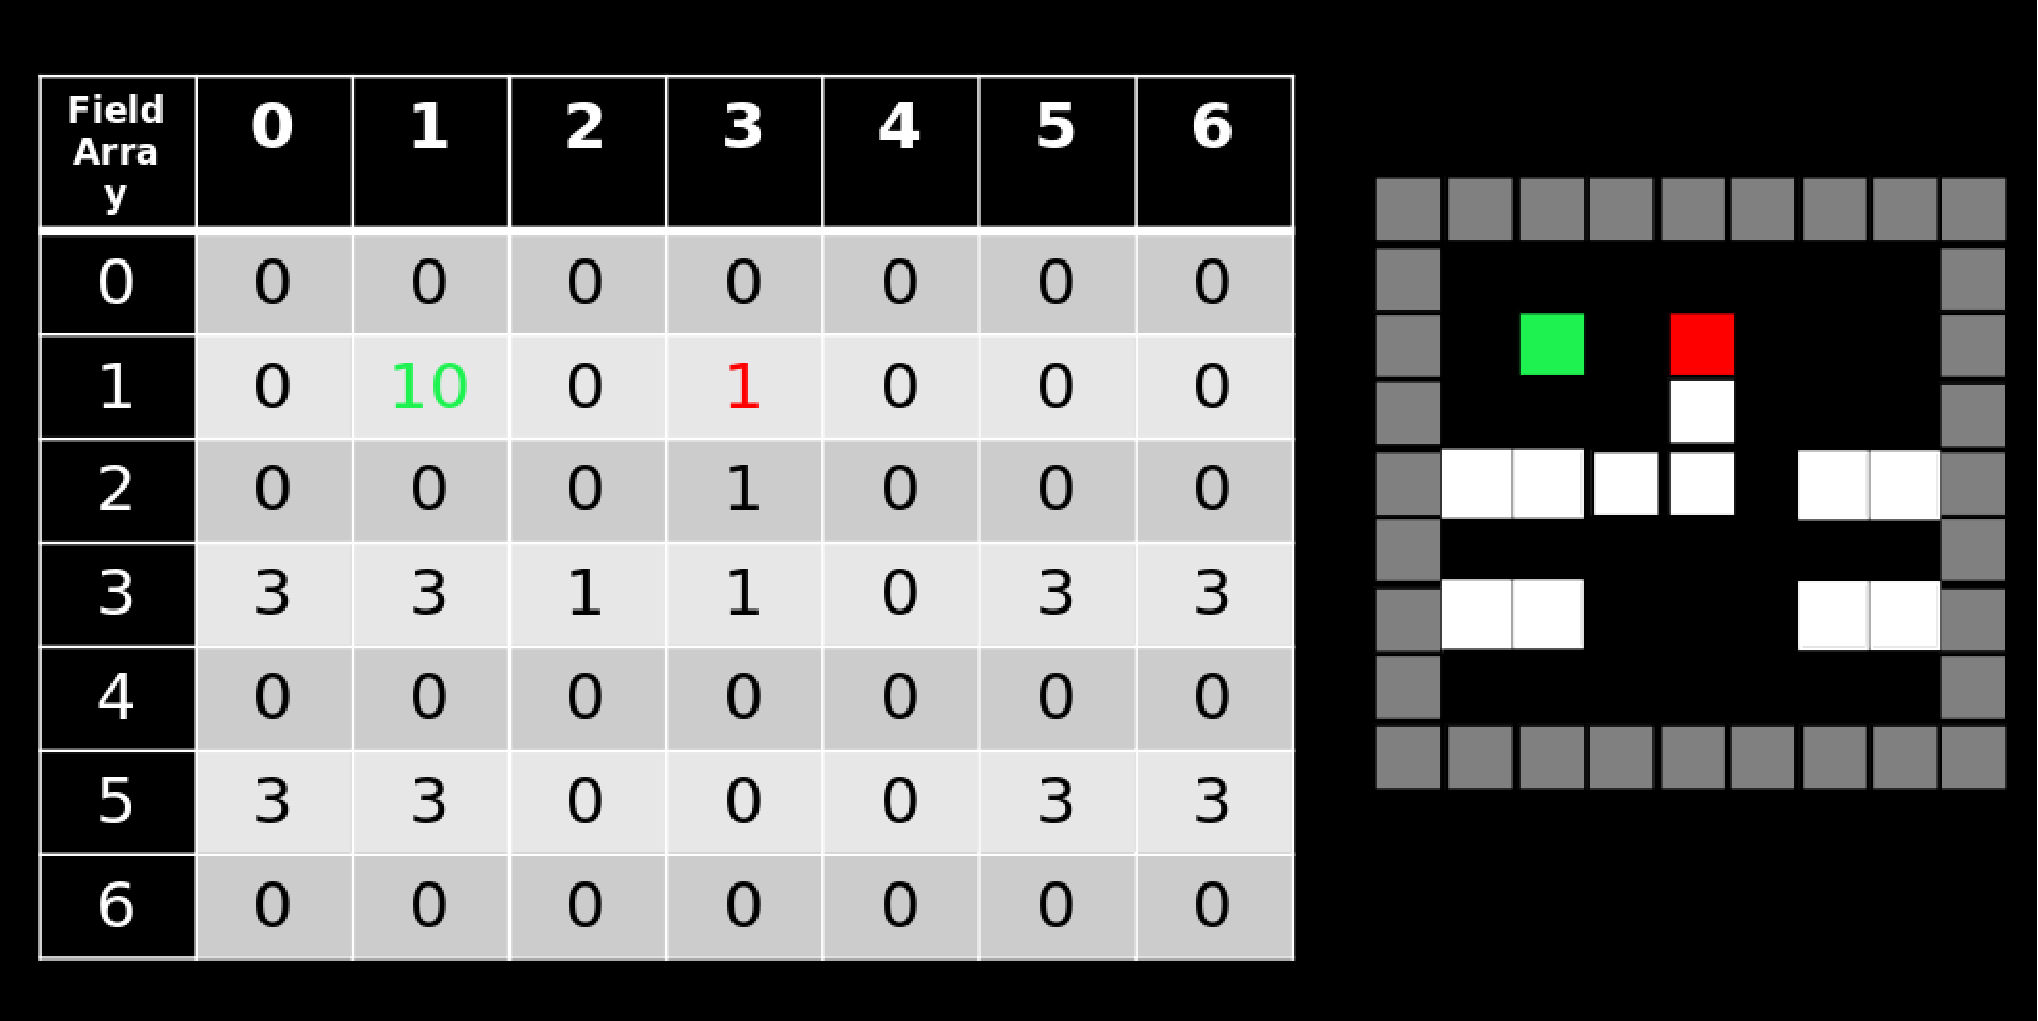
\includegraphics[scale=0.3]{bilder/FieldArraySpielfeld}
 \captionof{figure}{Darstellung des eines Spielfeldes mit dazugehörigem $fieldArray$}
 \label{fig:FieldArraySpielfeld}
\end{minipage}


\begin{table}
     \centering
     \begin{tabular}{ll}
       \textbf{Wert}  & \textbf{Objekt} \\
       0          & Leer                 \\
       1         & Spieler 1             \\
       2         & Spieler 2             \\
       3         & Wand                 \\
       10        & Food-Element             \\
       11        & Superfood-Element             \\
       12        & Freeze-Element             \\
       13        & Reduce-Element             \\
       14        & Inverse-Element             \\
       20        & Teleport             \\
     \end{tabular}

     \caption{Fieldarray-Werte}
     \label{tbl:Fieldarray-Werte}
     % Verweis im Text mittels \ref{tbl:beispieltabelle}

   \end{table}




%
\section{Spielleistung}
\label{Spielleistung}
%
Beim Ausf{\"u}hren des Spiels kam es sehr oft zu Problemen mit der Spielleistung. Insbesondere wenn das Spiel mit anderen Programmen, wie BigBlueButton, gleichzeitig lief. Dies f{\"u}hrte in den meisten F{\"a}llen zur Verlangsamung des Spielfluss. Desweiteren flackerte das Spiel sehr stark, sodass {\"a}ltere Frames anstatt des neuen Frames gezeichnet wurden. Weitere Probleme waren h{\"a}ufig auftretende Speicherzugriffsfehler vor allem, wenn das Spiel {\"u}ber eine virtuelle Maschine lief. Jener Fehler f{\"u}hrte zur Terminierung des Spiels.  
%


%\include{chapter/erklaerung.tex}
% Anhang ---------------------------------------------------------------
%
%\cleardoublepage
%\appendix


%\include{chapter/appendix}

% Abbildungsverzeichnis -------------------------------------------------
%
\listoffigures
\addcontentsline{toc}{chapter}{List of Figures }
%\cleardoublepage

% Algorithmenverzeichnis ------------------------------------------------
%
%\listofalgorithms
%\addcontentsline{toc}{chapter}{List of Algorithms}
%\cleardoublepage

% Quellcodeverzeichnis --------------------------------------------------
%
\renewcommand{\lstlistlistingname}{List of Source Codes}


\lstlistoflistings
\addcontentsline{toc}{chapter}{List of Source Codes}
\href{https://github.com/XgXGhostXgX/SnakeRTOSEmulator.git}{GitHub Repository}
%\cleardoublepage
% ----------------------------------------------------------------------


%\cleardoublepage
%\addcontentsline{toc}{chapter}{Eidesstattliche Versicherung}
%\include{Eidesstattliche_Versicherung.pdf}
%\clearpage
\pagestyle{empty}
\addcontentsline{toc}{chapter}{Eidesstattliche Versicherung}
\includegraphics[trim = 20mm 20mm 20mm 10mm, clip,
width=\textwidth]{Eidesstattliche_Versicherung.pdf}


%\include{chapter/appendix}

\end{document}
